\chapter{Los diferentes Steps y sus resultados (StepResult)} \label{sec:steps_detallados}
De manera predeterminada, Samplers provee los Steps que se explican a continuación. Además de los provistos por Samplers, un usuario programador puede definir y agregar sus propios Steps, junto con sus StepFragments y StepResults como se explica en la sección \ref{sec:definir_steps} 

Todos los Step tienen los siguientes campos:

\begin{itemize}
\item \textbf{id:} El identificador del Step, que debe ser único por instancia.
\item \textbf{type:} El tipo de Step, que debe ser uno de los que se detallan a continuación.
\item \textbf{nextStepId:} [Opcional] El identificador del siguiente Step que se debe ejecutar al finalizar con el actual. Si no se especifica, se asume que el Step es el final del Workflow.
\item \textbf{helpFileName:} [Opcional] El nombre del archivo HTML con la ayuda del Step (como se explicó en la sección \ref{sec:mostrar_ayuda}. Si no se especifica, no se mostrará el botón de ayuda para el Step.
\end{itemize}

Además de estos campos, los diferentes tipos de Step agregan campos adicionales como se detalla en la explicación de cada Step a continuación.


\section{PhotoStep: Tomar una foto}
PhotoStep se usa para solicitarle al científico ciudadano que tome una foto. Tiene un texto (text) que se muestran a modo de instrucciones o mensaje cuando la cámara esta encendida. Luego de tomada la foto, se muestra una vista preliminar de la misma, con un botón que da la opción de volver a tomar la foto.

\begin{figure}[H]
  \centering
    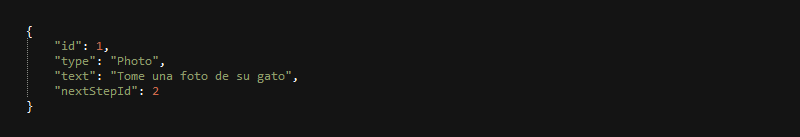
\includegraphics[scale=0.6]{50-anexos/C-steps/photo_json.png} 
    \caption{PhotoStep usando el generador de clases.}
\end{figure}	

\begin{figure}[H]
  \centering
    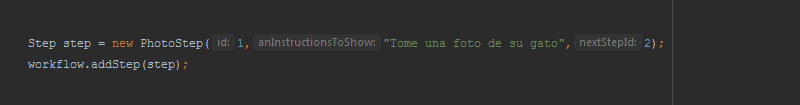
\includegraphics[scale=0.6]{50-anexos/C-steps/photo_java.png} 
    \caption{PhotoStep en Java.}
\end{figure}


\begin{figure}[H]
  \centering
    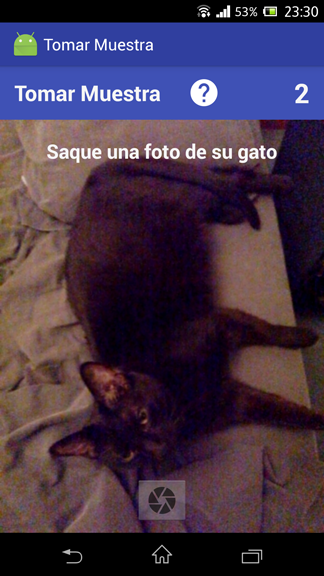
\includegraphics[scale=0.4]{05-implementacion/PhotoStep1.png} 
    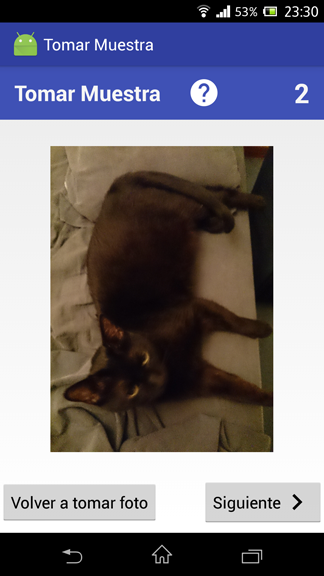
\includegraphics[scale=0.4]{05-implementacion/PhotoStep2.png}     
   \caption{Ejemplo de un PhotoStep en ejecución. A la izquierda al momento de tomar la foto, y a la derecha al momento de mostrar la vista preliminar.}
   \label{fig:imgPhotoStep}
\end{figure}

\subsection{PhotoStepResult: El resultado de Tomar una foto}
El PhotoStepResult contiene el nombre del archivo de la foto tomada. La foto va como archivo jpg en la carpeta de la muestra.
Puede haber varias fotos si hay varios PhotoSteps en el Workflow.




\section{SoundRecordStep: Grabar sonido}
SoundRecordStep  se usa para solicitarle al científico ciudadano que grabe un sonido. Tiene un texto (text) que se muestran a modo de instrucciones o mensaje. Luego de grabado el sonido, el mismo se puede escuchar, y en todo caso volver a grabar otro sonido.


\begin{figure}[H]
  \centering
    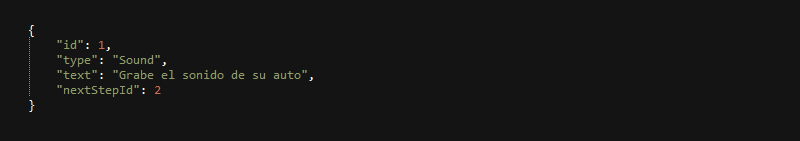
\includegraphics[scale=0.6]{50-anexos/C-steps/sound_json.png} 
    \caption{SoundRecordStep usando el generador de clases.}
\end{figure}	

\begin{figure}[H]
  \centering
    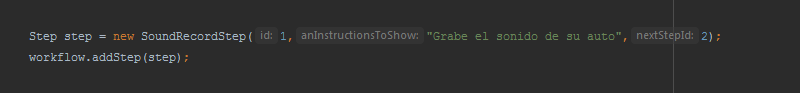
\includegraphics[scale=0.6]{50-anexos/C-steps/sound_java.png} 
    \caption{SoundRecordStep en Java.}
\end{figure}


\subsection{SoundRecordStepResult: El resultado de Grabar sonido}
El SoundRecordStepResult contiene el nombre del archivo del sonido grabado. El sonido va como archivo mp4 en la carpeta de la muestra.
Puede haber varios sonidos si hay varios SoundRecordSteps en el Workflow.



\section{InformationStep: Mostrar información}
InformationStep se usa para mostrar una información (texto) al científico ciudadano, por ejemplo, para mostrar un mensaje de bienvenida o para explicar brevemente los pasos que seguirán a continuación para tomar la muestra.


\begin{figure}[H]
  \centering
    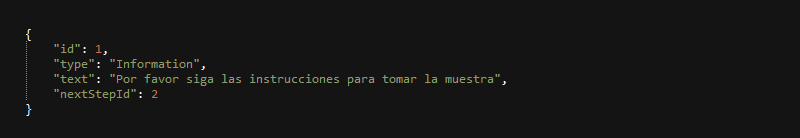
\includegraphics[scale=0.6]{50-anexos/C-steps/information_json.png} 
    \caption{InformationStep usando el generador de clases.}
\end{figure}	

\begin{figure}[H]
  \centering
    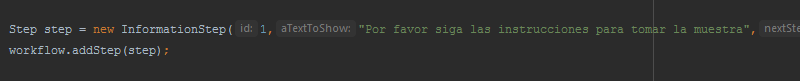
\includegraphics[scale=0.6]{50-anexos/C-steps/information_java.png} 
    \caption{InformationStep en Java.}
\end{figure}

\begin{figure}[H]
  \centering
    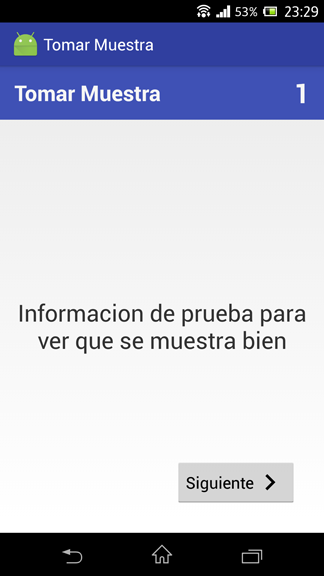
\includegraphics[scale=0.4]{05-implementacion/InformationStep.png} 
   \caption{Ejemplo de un InformationStep en ejecución}
   \label{fig:imgInformationStep}
\end{figure}


\subsection{InformationStepResult: El resultado de Mostrar información}
El resultado de mostrar información es nulo, es una clase vacía. Solo está para cerrar el circuito.





\section{SelectOneStep: Seleccionar una opción de un grupo de opciones}
SelectOneStep  se usa para solicitarle al científico ciudadano que seleccione una sola opción de varias opciones disponibles. Tiene un texto (title) que se muestran a modo de título o instrucciones. Las opciones disponibles para seleccionar son una lista de objetos SelectOneOption.
Cada objeto SelectOneOption tiene un id, textToShow y nextStepId, que se muestran en pantalla en forma de radio buttons.

Este caso particular de Step no tiene un identificador del siguiente Step a ejecutar (nextStepId), sino que cada opción seleccionable posee uno. Esto permite crear bifurcaciones en el Workflow, por ejemplo, se puede preguntar si se observa cierta característica y si la respuesta es si, pasar un PhotoStep para pedir que tome una foto de esa característica, pero si la respuesta es no, se puede saltar el paso de tomar una foto.

\begin{figure}[H]
  \centering
    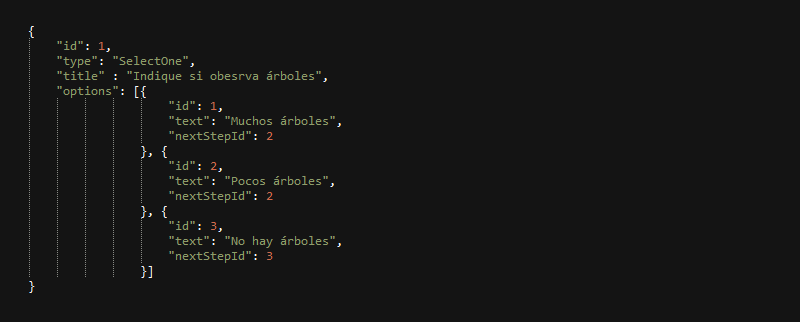
\includegraphics[scale=0.6]{50-anexos/C-steps/select_one_json.png} 
    \caption{SelectOneStep usando el generador de clases.}
\end{figure}	

\begin{figure}[H]
  \centering
    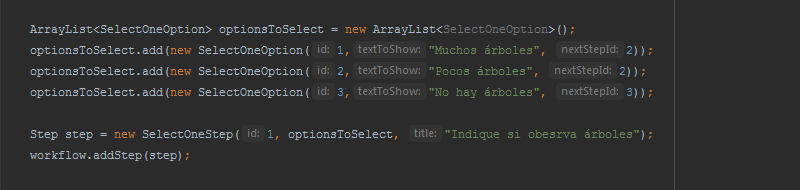
\includegraphics[scale=0.6]{50-anexos/C-steps/select_one_java.png} 
    \caption{SelectOneStep en Java.}
\end{figure}


\subsection{SelectOneStepResult: El resultado de Seleccionar una opción de un grupo de opciones}
SelectOneStepResult contiene la opción seleccionada (un objeto SelectOneOption).





\section{MultipleSelectStep: Seleccionar varias opciones de un grupo de opciones}
MultipleSelectStep  se usa para solicitarle al científico ciudadano que seleccione una o más opciones de varias opciones disponibles. Tiene un texto (title) que se muestran a modo de título o instrucciones. Las opciones disponibles para seleccionar son una lista de objetos MultipleSelectOption.
Cada objeto MultipleSelectOption tiene un id, textToShow.
Las opciones disponibles para seleccionar se muestran en pantalla en forma de check-boxes.


\begin{figure}[H]
  \centering
    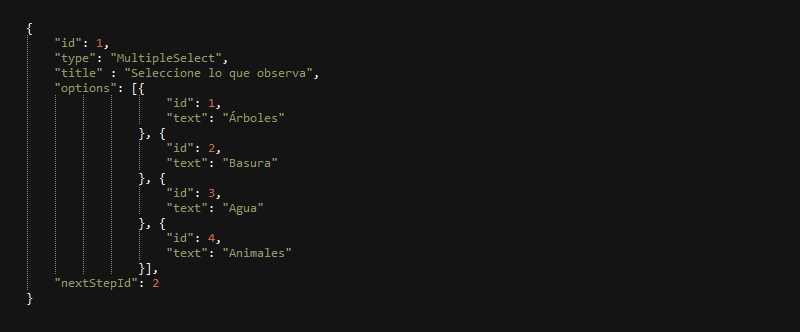
\includegraphics[scale=0.6]{50-anexos/C-steps/multiple_select_json.png} 
    \caption{MultipleSelectStep usando el generador de clases.}
\end{figure}	

\begin{figure}[H]
  \centering
    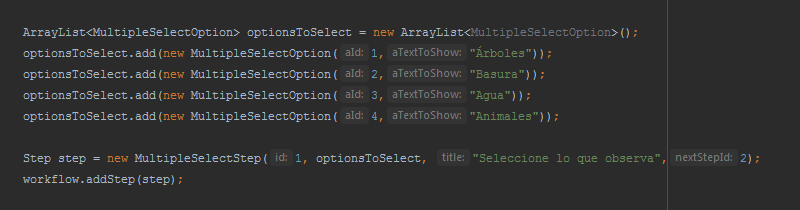
\includegraphics[scale=0.6]{50-anexos/C-steps/multiple_select_java.png} 
    \caption{MultipleSelectStep en Java.}
\end{figure}


\subsection{MultipleSelectStepResult: El resultado de Seleccionar varias opciones de un grupo de opciones}
MultipleSelectStepResult contiene una lista de las opciones seleccionadas (una lista de objetos MultipleSelectOption).





\section{LocationStep: Posicionar la muestra en el mapa con el GPS}
LocationStep se usa para solicitarle al científico ciudadano que tome la posición con el GPS del dispositivo móvil. Tiene un texto (textToShow) que se muestran a modo de instrucciones o mensaje. 

Permite usar el GPS o posicionar la muestra manualmente en el mapa.

En Android Studio (Java):
\begin{lstlisting}[language=Java, frame=tlb]	
LocationStep step = new LocationStep(1,"Por favor posicione la muestra en el mapa",2); 
\end{lstlisting}

Usando el generador de clases:
\begin{lstlisting}[language=XML, frame=tlb]	
{
  "id" : 1,
  "type" : "Location",
  "text" : "Por favor posicione la muestra en el mapa",
  "nextStepId" : 2
}
\end{lstlisting}

\subsection{LocationStepResult: El resultado de Posicionar la muestra en el mapa con el GPS}
LocationStepResult contiene la latitud y longitud (ambos de tipo double) de la posición GPS tomada.


\section{RouteStep: Grabar un recorrido en el mapa usando el GPS}
[falta desarrollar]
\begin{comment}
Tiene un textToShow a modo de instrucciones
Intervalo y mapZoom opcionales. Poner los valores por defecto
\end{comment}

En Android Studio (Java):
\begin{lstlisting}[language=Java, frame=tlb]	
RouteStep step = new RouteStep(1,"Registre la ruta que corre",2); 
step.setInterval(10000);
step.setMapZoom(18);
\end{lstlisting}

Usando el generador de clases:
\begin{lstlisting}[language=XML, frame=tlb]	
{
  "id" : 1,
  "type" : "Route",
  "text" : "Registre la ruta que corre",
  "interval" : 10000,
  "mapZoom" : 18,
  "nextStepId" : 2
}
\end{lstlisting}

\subsection{RouteStepResult: El resultado de Grabar un recorrido en el mapa usando el GPS}
[falta desarrollar]
%guarda una lista de objetos Location

\section{InsertTextStep: Ingresar texto}
[falta desarrollar]
\begin{comment}
textToShow a modo de instrucciones
sampleText a modo de ejmplo
maxLength cantidad máxima de caracteres permitida
Type Values allowed are: text, number or decimal
optional indicando si se puede dejar vacío y no ingresar ningún texto (true) o si se requiere que ingrese algo si o si (false)
\end{comment}



En Android Studio (Java):
\begin{lstlisting}[language=Java, frame=tlb]	
InsertTextStep step = new InsertTextStep(1,"Por favor, ingrese el nombre del lago","Nombre del lago",50,InsertTextStep.InputType.TYPE_TEXT,true,2);
\end{lstlisting}

Usando el generador de clases:
\begin{lstlisting}[language=XML, frame=tlb]	
{
  "id" : 1,
  "type" : "InsertText",
  "text" : "Por favor, ingrese el nombre del lago",
  "sampleText" : "Nombre del lago",
  "inputType" : "text",
  "maxLength" : 50,
  "optional" : true,
  "nextStepId" : 2
}
\end{lstlisting}

\subsection{InsertTextStepResult: El resultado de Ingresar texto}
[falta desarrollar]
%guarda el texto ingresado en insertedText

\section{InsertDateStep y InsertTimeStep: Ingresar fecha y hora}
[falta desarrollar]
\begin{comment}
ambos tienen textToShow a modo de instrucciones
\end{comment}


En Android Studio (Java):
\begin{lstlisting}[language=Java, frame=tlb]	
InsertDateStep step = new InsertDateStep(1,"Por favor indique la fecha de la muestra",2); 
\end{lstlisting}

Usando el generador de clases:
\begin{lstlisting}[language=XML, frame=tlb]	
{
  "id" : 1,
  "type" : "InsertDate",
  "text" : "Por favor indique la fecha de la muestra",
  "nextStepId" : 2
}
\end{lstlisting}

En Android Studio (Java):
\begin{lstlisting}[language=Java, frame=tlb]	
InsertTimeStep step6 = new InsertTimeStep(1,"Por favor indique la hora de la muestra",2); 
\end{lstlisting}

Usando el generador de clases:
\begin{lstlisting}[language=XML, frame=tlb]	
{
  "id" : 1,
  "type" : "InsertTime",
  "text" : "Por favor indique la hora de la muestra",
  "nextStepId" : 2
}
\end{lstlisting}

\subsection{InsertDateStepResult y InsertTimeStep: El resultado de Ingresar fecha y hora}
[falta desarrollar]
%un objeto Date que tiene la fecha o la hora según corresponda



\section{Definir un nuevo Step, StepFragment y StepResult} \label{sec:definir_steps}
[acá vamos a explicar como definir un nuevo Step para extender el framework]



